% -----------------------------*- LaTeX -*------------------------------
\documentclass[11pt]{report}
\usepackage{epstopdf}
\usepackage{hw_style}
\usepackage{graphicx}
\usepackage{dsfont}
\usepackage{caption}
\usepackage{subcaption}


\def\exp#1{\mathop{\mathrm{exp}}\left( #1\right)}
\usepackage{amsmath}
\begin{document}
\scribe{Ankush Gupta} % required
\hwnumber{1} % required, must be a number
\duedate{Feb 25} % required, omit year
\maketitle
% ----------------------------------------------------------------------
\subsection*{Introduction}
In this lab we investigate using Gaussian Processes for regression on weather data prediction. Following are the main features of this implementation.
\begin{itemize}
    \item The code was implemented in Python.
    \item Two mean functions were analyzed : (1) constant mean = mean of the data (2) cubic spline fit to the data.\footnote{ Note that these are strictly not bayesian methods as we are using the data itself to specify the prior.}
    \item Two covariance functions were analyzed :
        \begin{enumerate}
        \item Squared-Exponential = $\sigma^2 exp\left(-\dfrac{(x_1-x_2)^TM^{-1}(x_1-x_2}{2}\right) + \sigma_y^2I$
        \item Periodic  = $\sigma^2 exp\left(-l^2\sin^2(2\pi/b|x_1-x_2|)\right)$
        \end{enumerate}
        \item The hyperparameters were tuned by maximizing the marginal likelihood. Analytical gradients were used with the conjugate gradient optimization method.
        \item Sequential predictions were also carried out for Tide Height and Temperature time series.
\end{itemize}
\textbf{Please note all figures indicate intervals of 1 and 2 standard deviations.}
\subsection*{RMS Error with Different Means/ Covariances}
The table below indicates the root-mean-squared error of the \textbf{tide-height} predcitions with respect to the ground-truth data. The covariance hyper-parameters used for these experiments were optimised through marginal likelihood as detailed in the next section.

\begin{table}[h]
\begin{center}
\begin{tabular}{|l||r|r|r|r|r|r|r|r|r|r|r|}
\hline
Mean \textbackslash Covariance & Squared-Exponent & Periodic\\\hline\hline
Mean(data) & \textbf{0.158} &   0.175 \\\hline
Spline     & 0.240 &   0.290 \\\hline
\end{tabular}
\caption{RMS Error for tide-height predictions.}
\label{tab1}
\end{center}
\end{table}Note that the root-mean squared error is the lowest for squared-exponential with the mean function equal to the mean of the output. However, if we observe the plots in Figure~\ref{fig:f1}, we note that the variance in the predictions in the region with no observations (beyond t=7000), is lower for the periodic covariance. This is because the periodic covariance is able to capture the long-term periodic trend in tide-height data, which the squared-exponent is unable to; the square-exponent predicitions converge to the estimate of the mean function with the variance being equal to the sum of signal variance and observation variance.

\begin{figure}[h]
\begin{subfigure}[h]{\linewidth}
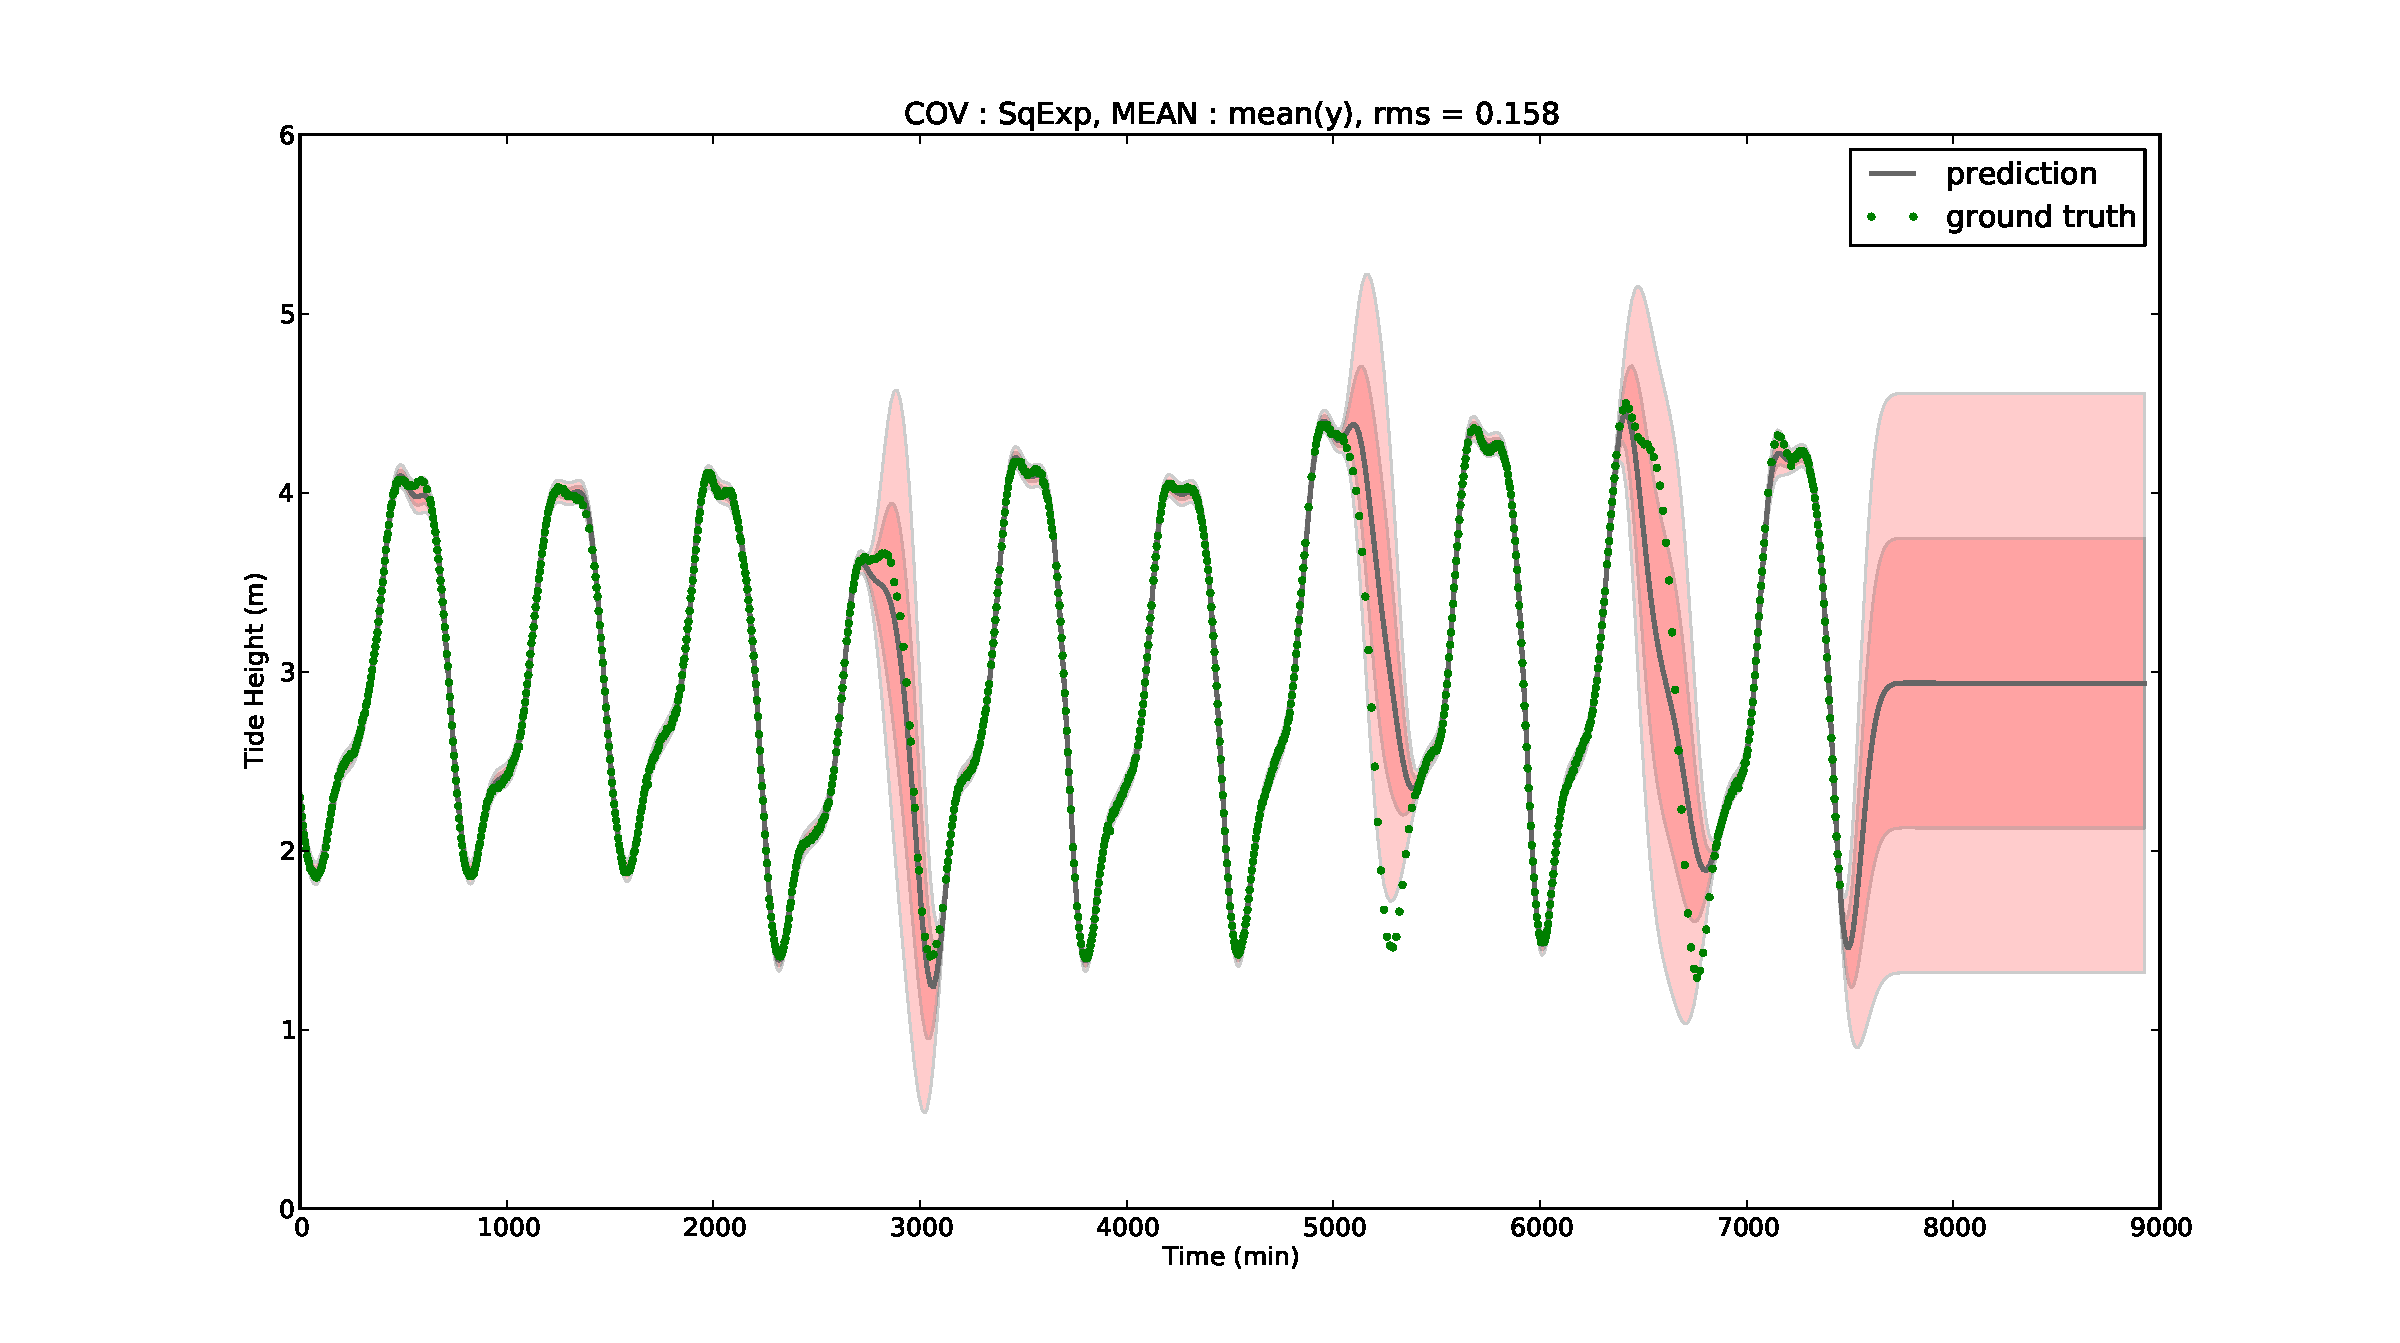
\includegraphics[width=15cm, height=6.5cm]{figs/h_sqexp_const.pdf}
\caption{}
\end{subfigure}\\
\begin{subfigure}[h]{\linewidth}
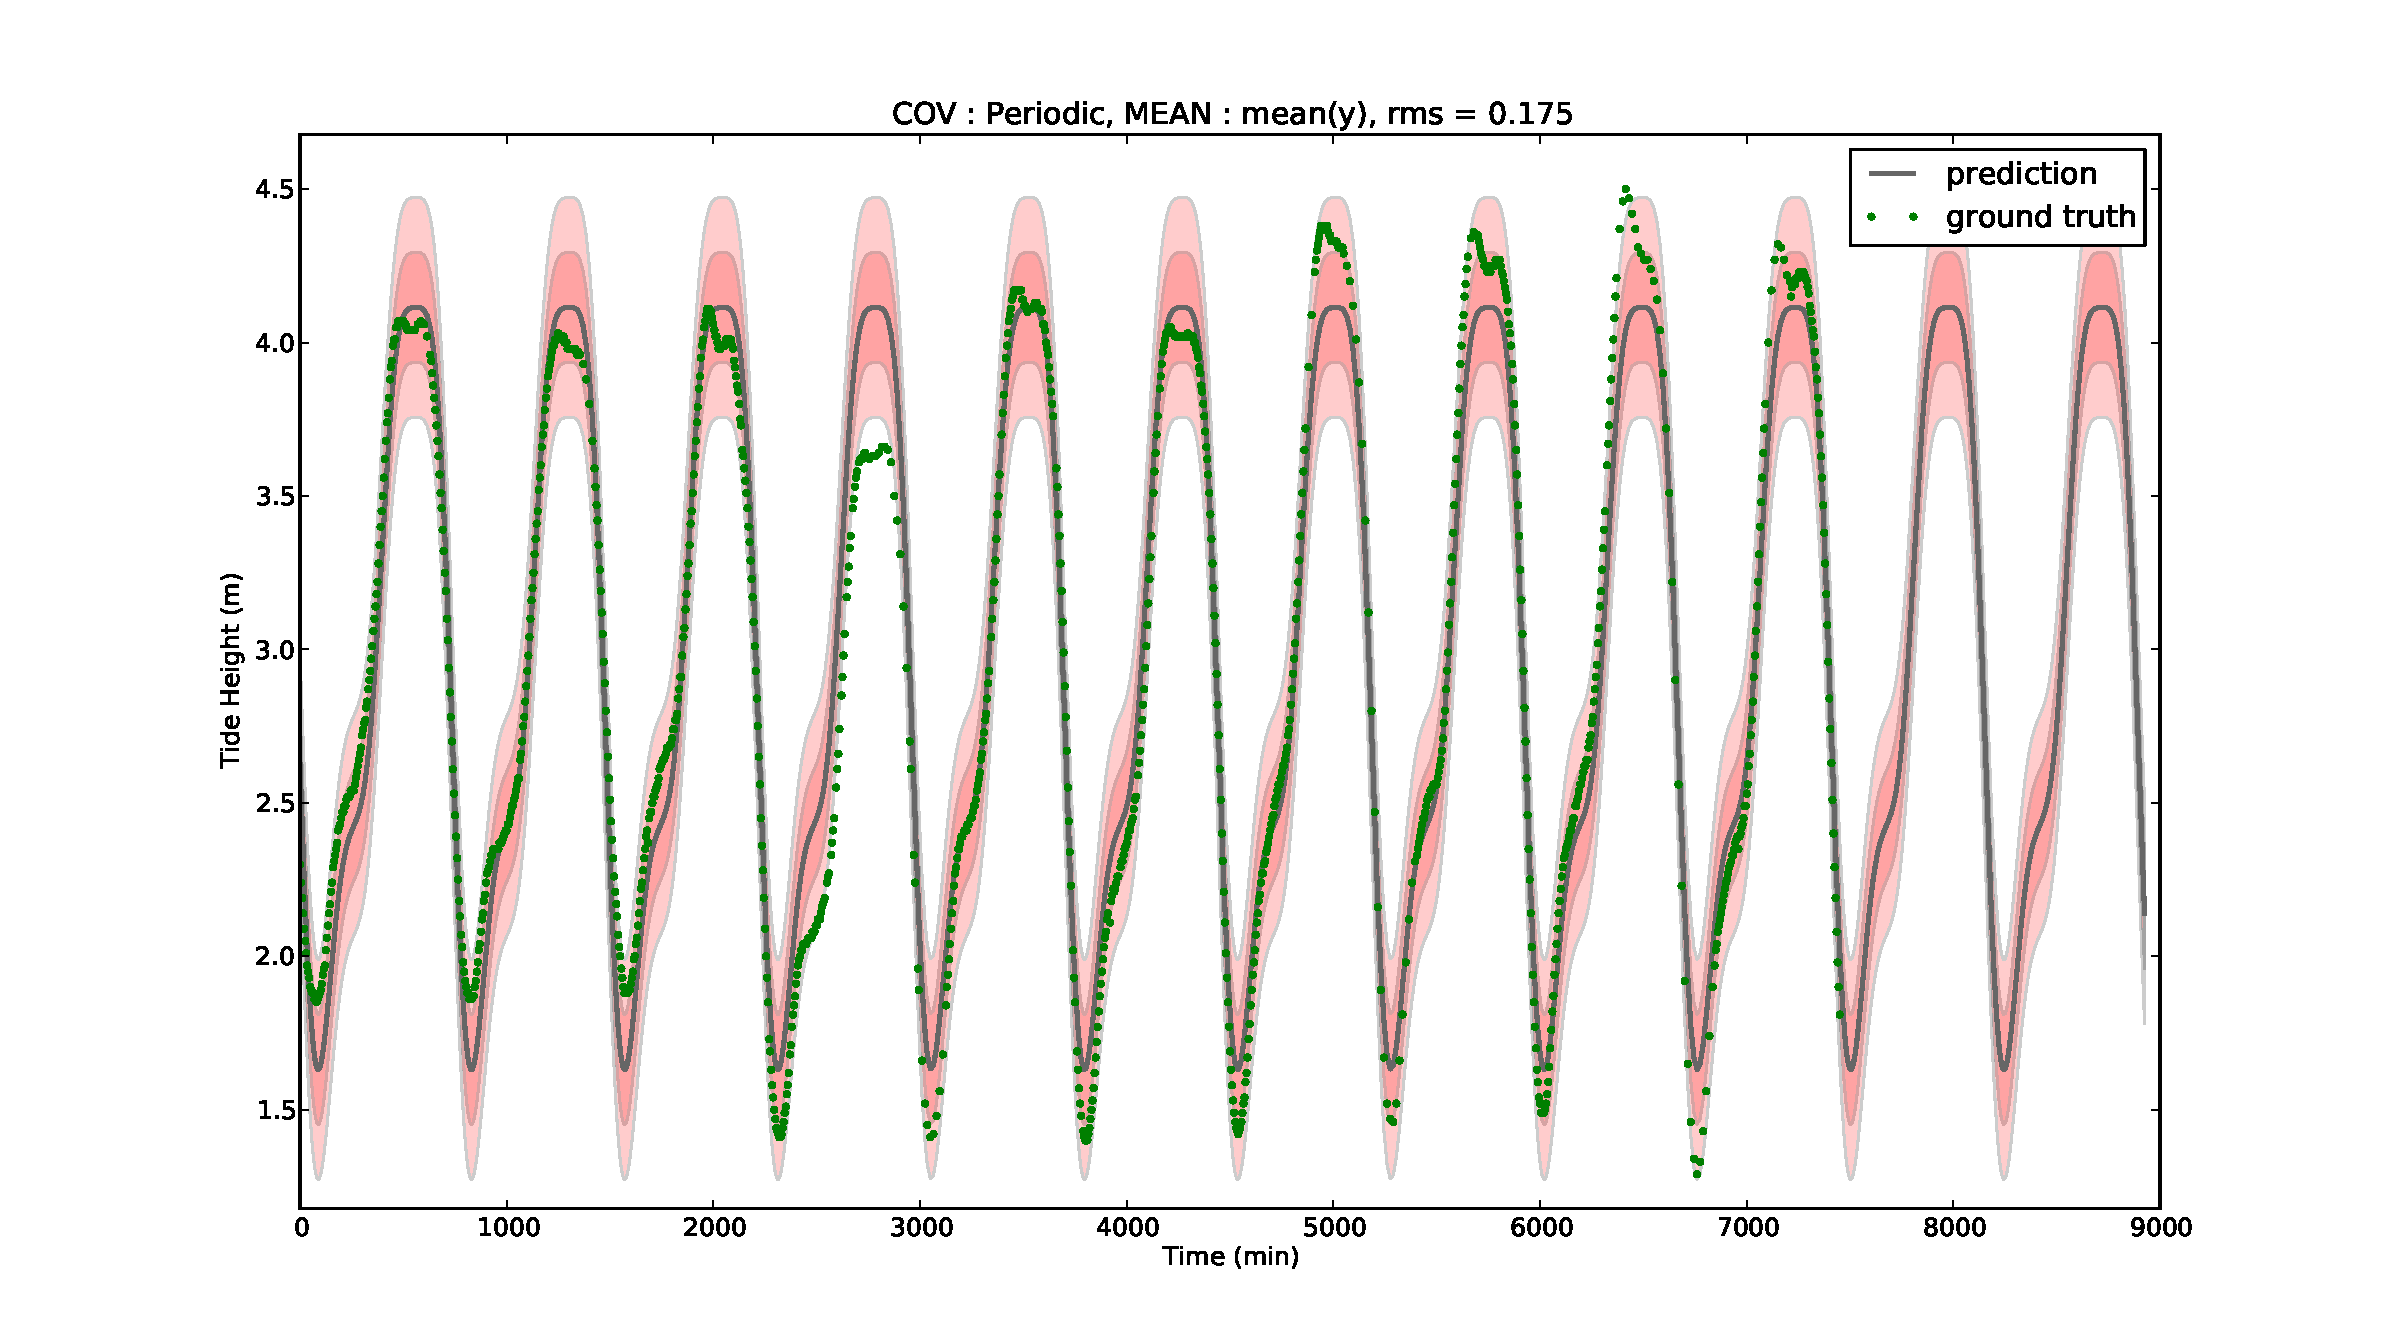
\includegraphics[width=15cm, height=6.5cm]{figs/h_per_const.pdf}
\caption{}
\end{subfigure}%
\caption[]{The figure (a) above uses the square-exponential covariance where as figure (b) uses periodic (sin-squared-exponent). Even though the rms error of (a) is lower than (b) (0.158 < 0.175), notice the variance towards the end (after $t>7000$) --- the variance for the squared-exponent is higher than periodic kernel because it cannot capture the long-term periodic trend in the data.}
\label{fig:f1}
\end{figure}
\clearpage

Below is a table similar to Table~\ref{tab1}, for the \textbf{temperature data series}. Since there is no long-term periodic trend, only the square-exponent kernel was used. We note that the constant mean function achieves a lower rms error.

\begin{table}[b]
\begin{center}
\begin{tabular}{|l||r|r|r|r|r|r|r|r|r|r|r|}
\hline
Mean \textbackslash Covariance & Squared-Exponent \\\hline\hline
Mean(data) & \textbf{0.541} \\\hline
Spline     & 1.954\\\hline
\end{tabular}
\caption{RMS Error for temperature predictions.}
\label{tab2}
\end{center}
\end{table}
\subsection*{Determining the Hyper-parameters}
The hyper parameters were determined by minimising the negative marginal log likelihood of the data. The gradient of negative-log-likelihood (NLL) was calculated analytically using the expression $= \dfrac{1}{2}Tr\left( (K_y^{-1}yy^TK_y^{-T} - K_y^{-1}) \dfrac{\partial K_y}{\partial \theta_j}\right)$. The actual optimisation was done using the the Conjugate-Gradient method of the\texttt{scipy.optimize.minimize} function.\\

Figure~\ref{fig:f2} shows the NLL of the tide-height data as a function of $\log(b)$ and $\log(\sigma_n)$ --- the hyper-parameters in the square-exponent kernel $K(x_1,x_2)= \sigma^2exp(-1/2|(x_1-x_2)/b|) + \sigma_n^2I$. In this plot, $\sigma$ is held constant at its optimal value (which was found by minimising jointly over all three hyper-parameters). Gradient descent correctly found the minimum indicated in the figure.

\begin{figure}[h]
\begin{center}
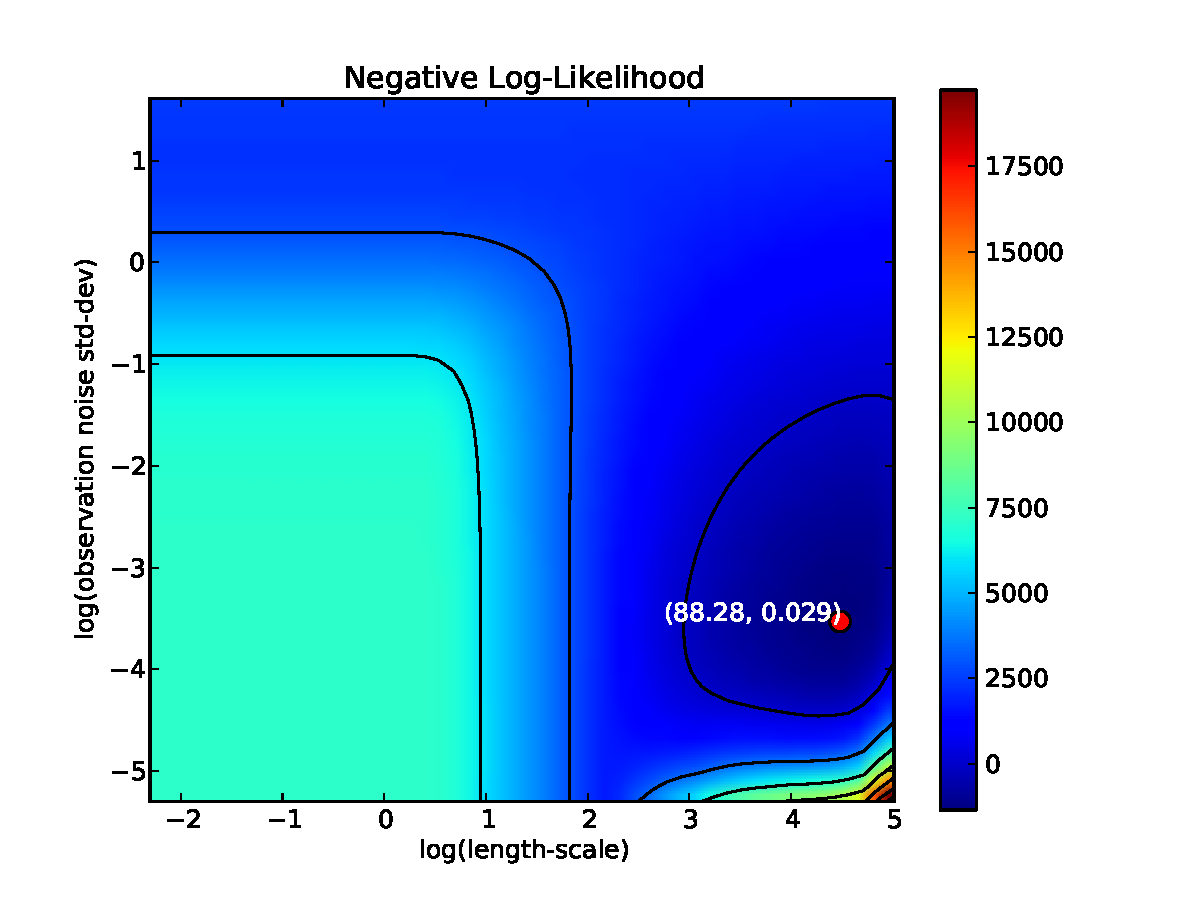
\includegraphics[width=10cm]{figs/nll.pdf}
\caption{Negative-log-likelihood of tide-height data-series as a function of two of the hyper parameters of the square-exponential kernel. Red point marked achieves the minimum.}
\label{fig:f2}
\end{center}
\end{figure}
\clearpage

\subsection*{Sequential Prediction}
Figure~\ref{f3} shows the result of making predictions sequentially. The key-feature here is that the variance incases as the time-gap since the last observations increases and suddenly decreases when an observations is made.
\begin{figure}[h]
\begin{subfigure}[h]{\linewidth}
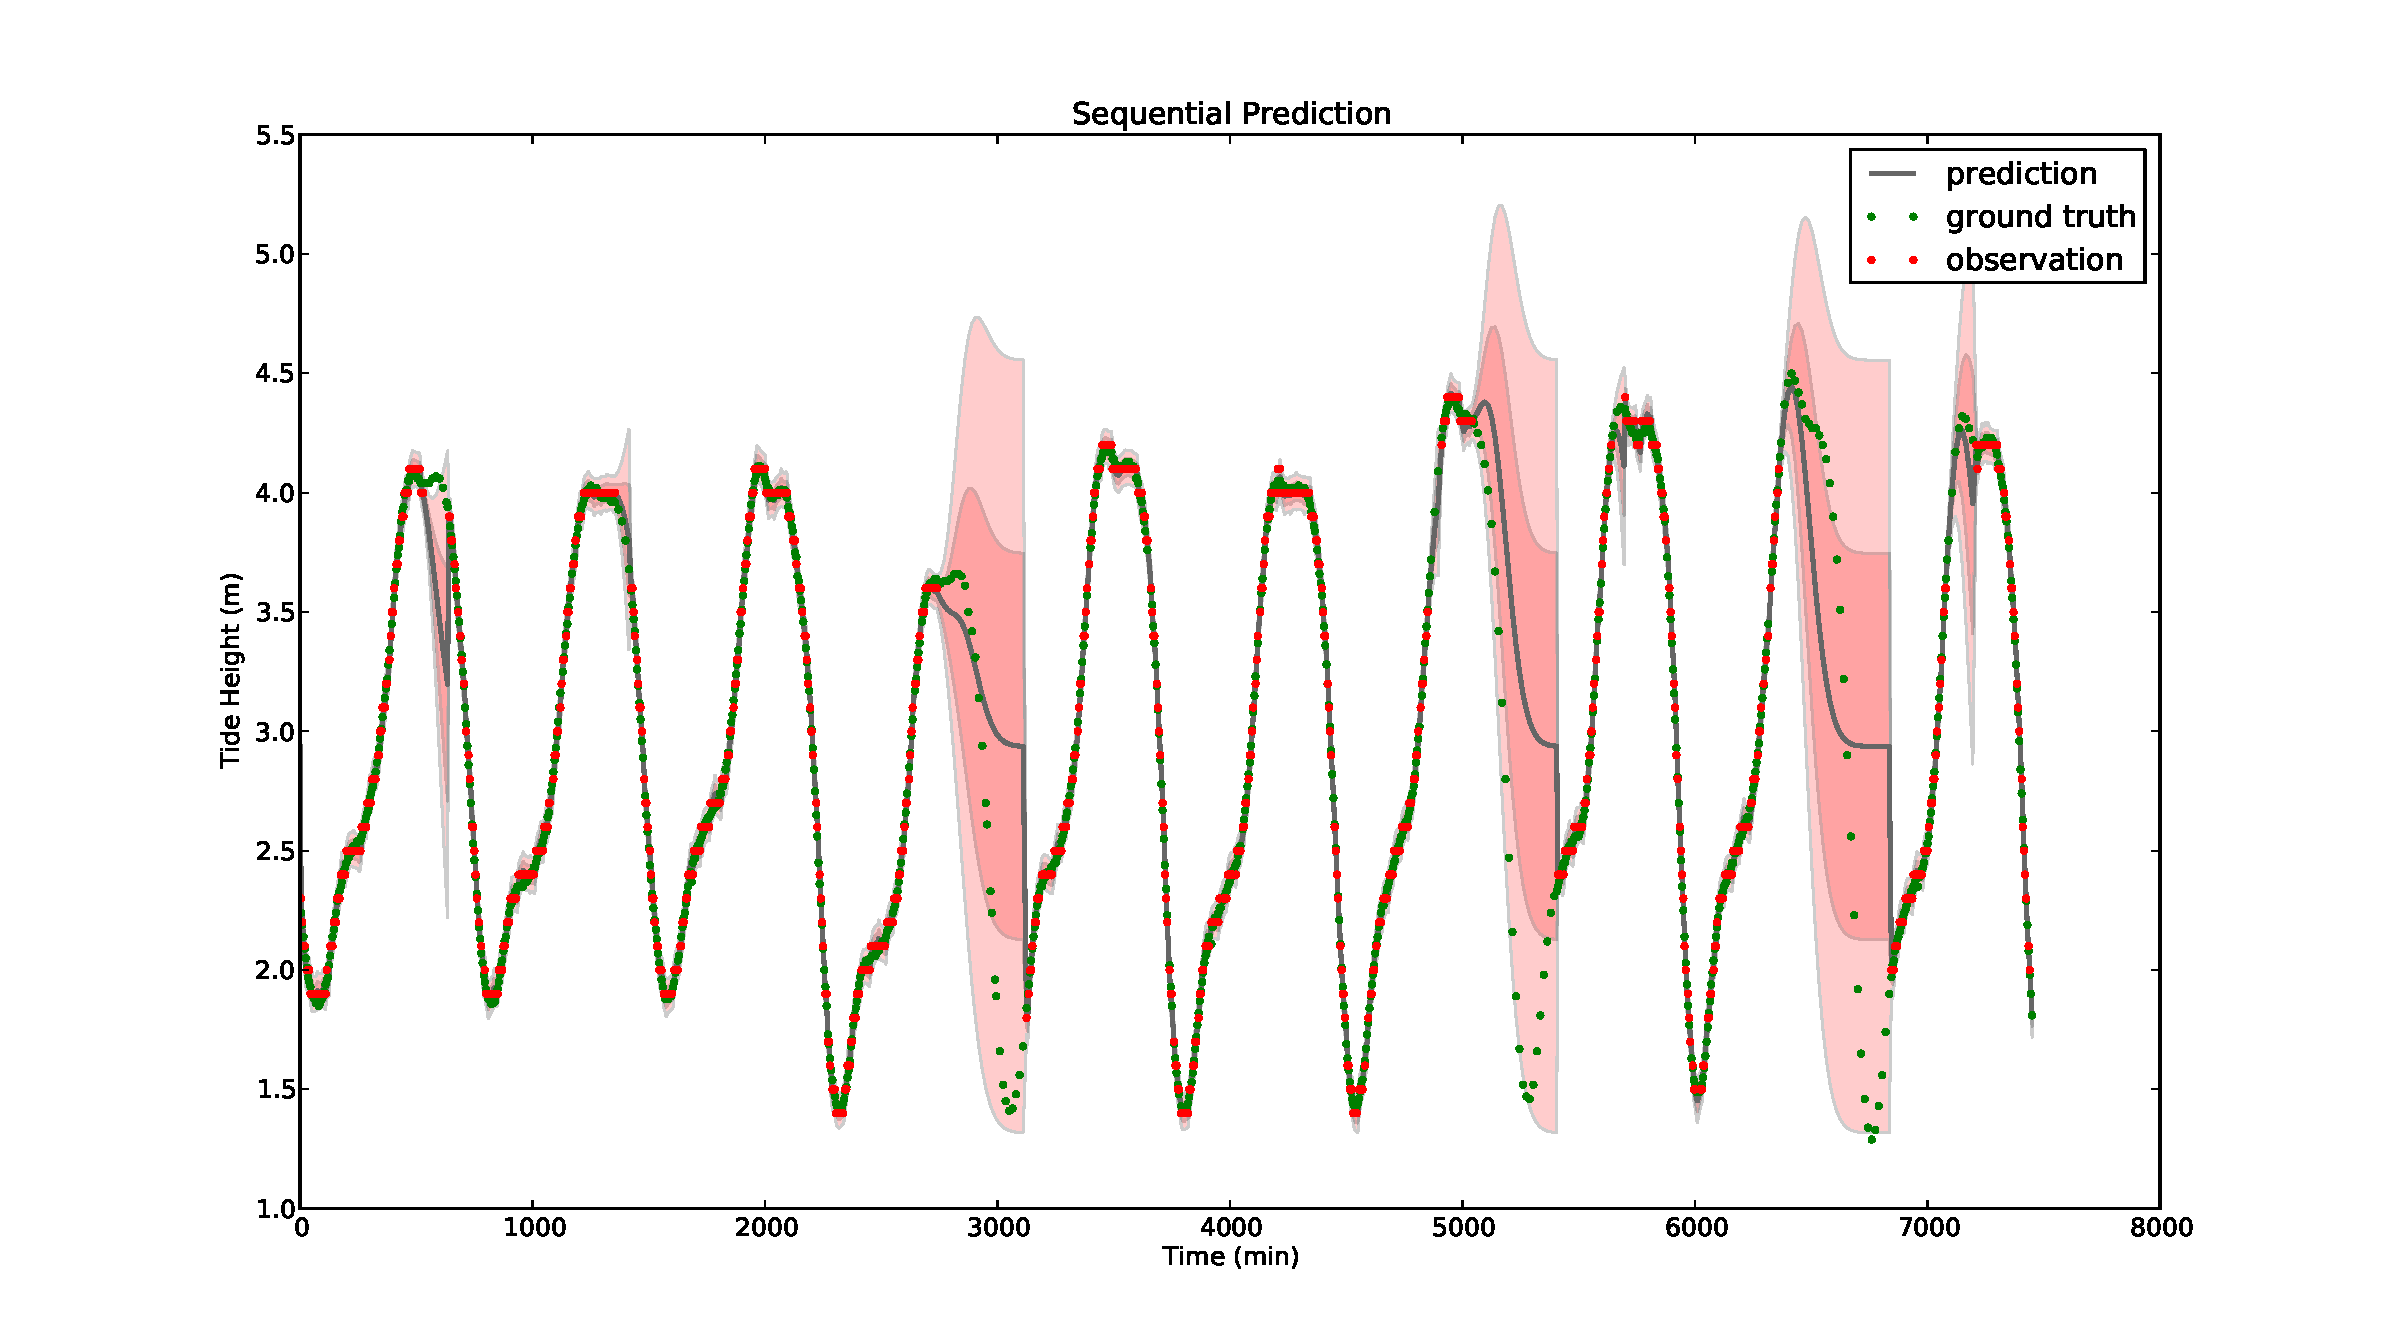
\includegraphics[width=15cm, height=7cm]{figs/h_seq.pdf}
\end{subfigure}\\
\begin{subfigure}[h]{\linewidth}
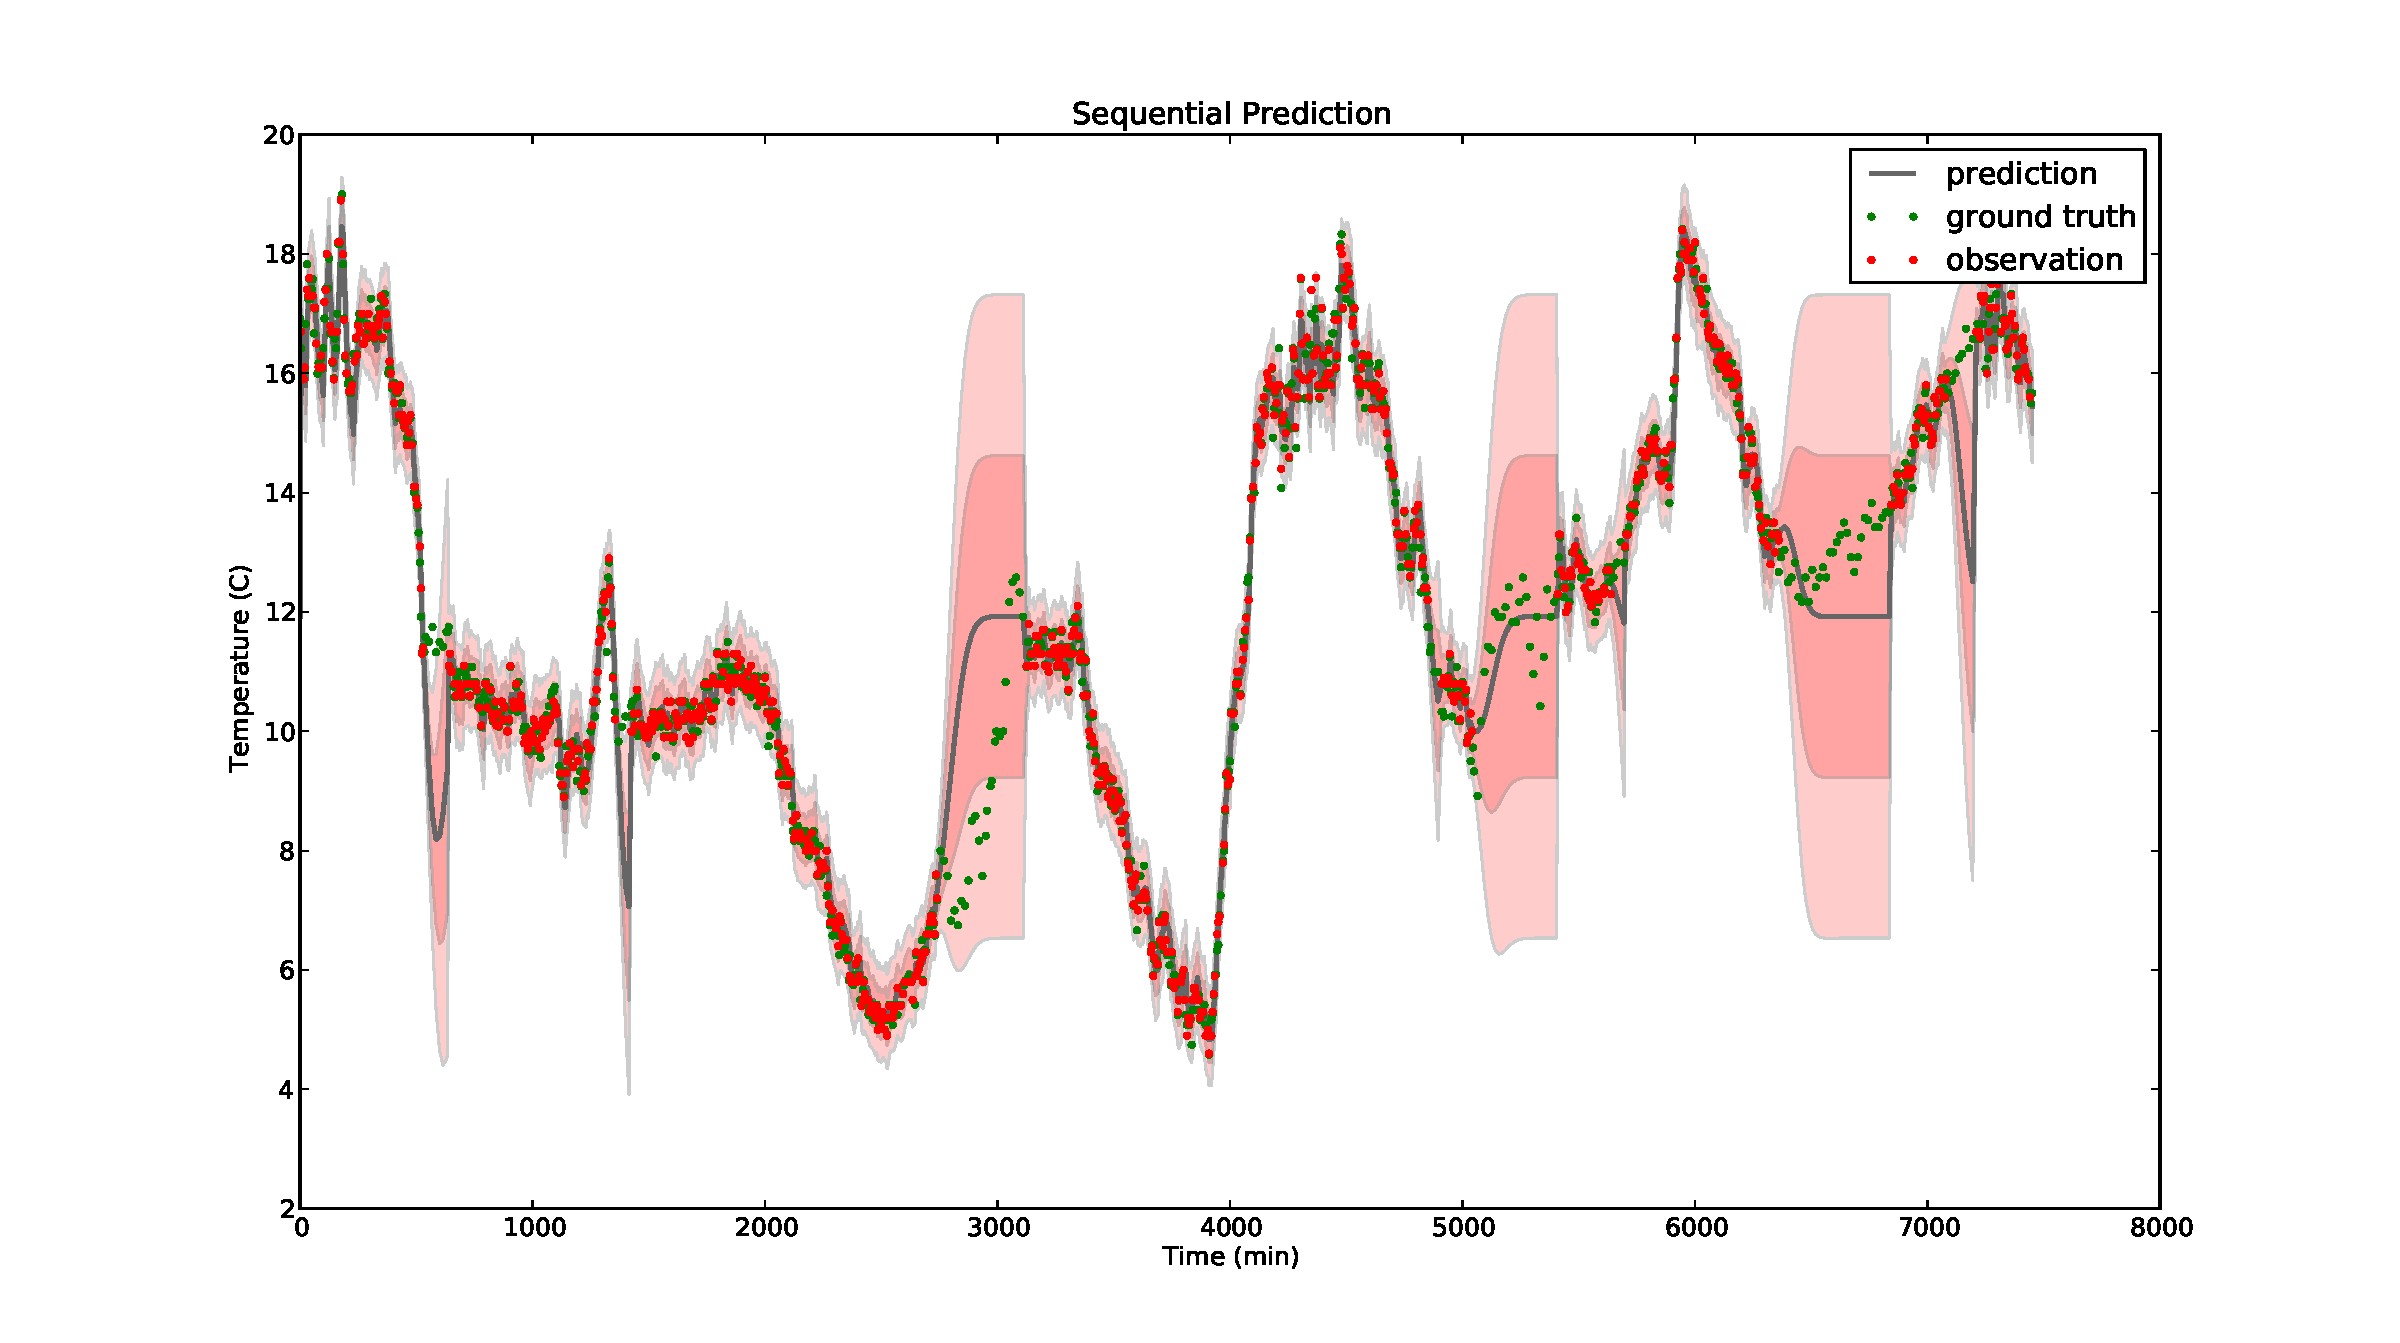
\includegraphics[width=15cm, height=7cm]{figs/T_seq.pdf}
\end{subfigure}%
\caption{\textbf{Sequential prediction} : [Top] Tide Height. [Bottom] Temperature.}
\label{f3}
\end{figure}
\clearpage
\subsection*{Future Consideration}
I tried to get a generic class working --- one which could taking any two existing kernels and produce a new one by multiplying them together. This could be used in capturing the local periodicity in the temperature data by multiplying the squared-exponential and the periodic kernel. Unfortunately, I faced numerical problems when optimising for hyper-parameters --- which could not be resolved in the time I had. I would like to work on this further in the future and see if it can improve the performance.
\end{document}
